\documentclass[12pt, a4paper]{article}
\usepackage[utf8]{inputenc}
\usepackage[T1]{fontenc}
\usepackage{lmodern}
\usepackage[spanish, es-nodecimaldot, es-tabla]{babel}
\usepackage[top=2.25cm, bottom=2cm, left=3cm, right=2.5cm]{geometry}
\usepackage[style=ieee, backend=biber, sorting=none, doi=true]{biblatex}
\usepackage{setspace}
\onehalfspacing
\setlength{\parindent}{1.25cm}
\setlength{\parskip}{2pt}
\usepackage{titlesec}
\titleformat{\section}{\large\bfseries}{\thesection.}{0.5em}{}
\titleformat{\subsection}{\normalsize\bfseries}{\thesubsection.}{0.5em}{}
\titleformat{\subsubsection}{\normalsize\itshape}{\thesubsubsection.}{0.5em}{}
\titlespacing{\section}{0pt}{14pt}{6pt}
\titlespacing{\subsection}{0pt}{10pt}{4pt}
\titlespacing{\subsubsection}{0pt}{8pt}{3pt}
\usepackage{booktabs}
\usepackage{array}
\usepackage{float}
\usepackage{graphicx}
\usepackage{caption}
\captionsetup{font=small, labelfont=bf, skip=6pt}
\usepackage[hidelinks, breaklinks=true]{hyperref}
\usepackage{url}
\urlstyle{tt}
\usepackage{fancyhdr}
\fancyhf{}
\fancyhead[L]{Aplicaciones Distribuidas \textperiodcentered{} UTEQ}
\fancyhead[R]{\small Cristhian Daniel Pacheco Cárdenas}
\fancyfoot[C]{\thepage}
\renewcommand{\headrulewidth}{0.4pt}
\setlength{\headheight}{14pt}
\usepackage[framemethod=default]{mdframed}
\usepackage{xcolor}
\definecolor{azulUTEQ}{RGB}{13, 42, 93}
\definecolor{grisClaro}{RGB}{245, 245, 245}
\definecolor{azulClaro}{RGB}{232, 240, 254}
\usepackage{enumitem}
\setlist[itemize]{noitemsep, topsep=3pt, leftmargin=1.4em}
\setlist[enumerate]{noitemsep, topsep=3pt, leftmargin=1.6em}

\usepackage{filecontents}
\begin{filecontents*}{referencias.bib}
@article{abadi2012,
  author  = {Abadi, Daniel J.},
  title   = {Consistency Tradeoffs in Modern Distributed Database System Design: {CAP} is Only Part of the Story},
  journal = {Computer},
  volume  = {45},
  number  = {2},
  pages   = {37--42},
  year    = {2012},
  doi     = {10.1109/MC.2012.33}
}
@article{corbett2013,
  author  = {Corbett, James C. and others},
  title   = {Spanner: Google's Globally Distributed Database},
  journal = {ACM Transactions on Computer Systems},
  volume  = {31},
  number  = {3},
  pages   = {1--22},
  year    = {2013},
  doi     = {10.1145/2491245}
}
@inproceedings{decandia2007,
  author    = {DeCandia, Giuseppe and others},
  title     = {Dynamo: Amazon's Highly Available Key-value Store},
  booktitle = {Proceedings of the 21st ACM SIGOPS Symposium on Operating Systems Principles (SOSP '07)},
  pages     = {205--220},
  year      = {2007},
  doi       = {10.1145/1294261.1294281}
}
@article{gilbertlynch2002,
  author  = {Gilbert, Seth and Lynch, Nancy},
  title   = {Brewer's Conjecture and the Feasibility of Consistent, Available, Partition-Tolerant Web Services},
  journal = {ACM SIGACT News},
  volume  = {33},
  number  = {2},
  pages   = {51--59},
  year    = {2002},
  doi     = {10.1145/564585.564601}
}
@article{viottivukolic2016,
  author  = {Viotti, Paolo and Vukoli\'{c}, Marko},
  title   = {Consistency in Non-Transactional Distributed Storage Systems},
  journal = {ACM Computing Surveys},
  volume  = {49},
  number  = {1},
  pages   = {1--34},
  year    = {2016},
  doi     = {10.1145/2926965}
}
@inproceedings{terry1994,
  author    = {Terry, Douglas B. and Demers, Alan J. and Petersen, Karin and Spreitzer, Mike and Theimer, Marvin and Welch, Brent B.},
  title     = {Session Guarantees for Weakly Consistent Replicated Data},
  booktitle = {Proceedings of the 3rd International Conference on Parallel and Distributed Information Systems (PDIS)},
  pages     = {140--149},
  year      = {1994},
  doi       = {10.1109/PDIS.1994.331722}
}
@book{vansteen2017,
  author    = {van Steen, Maarten and Tanenbaum, Andrew S.},
  title     = {Distributed Systems},
  edition   = {3rd},
  publisher = {distributed-systems.net},
  year      = {2017},
  isbn      = {978-1543057386}
}
\end{filecontents*}
\addbibresource{referencias.bib}

\begin{document}

\begin{titlepage}
\centering
\vspace*{0.5cm}
{\large\bfseries Universidad Técnica Estatal de Quevedo}\\[6pt]
{\normalsize Facultad de Ciencias de la Computación}\\[4pt]
{\normalsize Carrera de Ingeniería de Software}

\vspace{1cm}
\rule{\linewidth}{1pt}\\[10pt]
{\Large\bfseries
  Análisis Crítico del Modelo de Consistencia y Replicación\\[4pt]
  en Bases de Datos Distribuidas:\\[4pt]
  Caso del Sistema de Gestión de Solicitudes de\\[4pt]
  Soporte Técnico de Internet (Equipo ACC)
}
\vspace{2pt}
\rule{\linewidth}{1pt}

\vspace{1.2cm}
{\normalsize
  \textbf{Código:} TA-IND-02\\[4pt]
  \textbf{Nombre:} Cristhian Daniel Pacheco Cárdenas\\[4pt]
  \textbf{Equipo PFC:} ACC -- Soporte Técnico ISP\\[4pt]
  \textbf{Asignatura:} Aplicaciones Distribuidas (ISR-701)\\[4pt]
  \textbf{Unidad:} 3 -- Bases de Datos Distribuidas\\[4pt]
  \textbf{Tipo de actividad:} Trabajo autónomo individual sumativo\\[4pt]
  \textbf{Período académico:} Regular 2026--2027 SPA\\[4pt]
  \textbf{Semestre:} Séptimo Semestre\\[4pt]
  \textbf{Docente:} Gleiston Cicerón Guerrero Ulloa\\[4pt]
  \textbf{Repositorio del PFC:} \url{https://github.com/CristhianP03/TA-IND-02-Informe-Tecnico-Individual}
}

\vspace{2.2cm}
{\small Quevedo, Ecuador \textperiodcentered{} 15 de julio de 2026}
\end{titlepage}

\pagestyle{fancy}

\section*{Resumen}
\addcontentsline{toc}{section}{Resumen}
El presente informe analiza el modelo de consistencia y la estrategia de replicación implementados en el Sistema de Gestión de Solicitudes de Soporte Técnico de Internet, desarrollado por el equipo ACC. A partir de la arquitectura de microservicios documentada, se identifica que la sincronización entre \texttt{ticket-service} y \texttt{report-service}, mediante el patrón CQRS y el bus de eventos Apache Kafka, constituye el objeto central de análisis en términos de replicación y consistencia. Se caracteriza dicho modelo como de consistencia eventual y se clasifica bajo el marco PACELC como PA/EL, priorizando disponibilidad ante particiones y latencia en operación normal. Se contrasta el modelo actual con dos alternativas --consulta síncrona directa y replicación multi-líder por quorum-- mediante criterios técnicos explícitos. La discusión crítica concluye que el modelo es adecuado para la ruta operativa del cliente, pero presenta una limitación real en el subdominio de reportes de cumplimiento de SLA, para la cual se proponen mitigaciones concretas.

\vspace{0.5cm}

% ============================================================
% 1. INTRODUCCIÓN
% ============================================================
\section{Introducción}
El Sistema de Gestión de Solicitudes de Soporte Técnico de Internet, desarrollado por el equipo ACC como Proyecto Fin de Curso (PFC) de la asignatura Aplicaciones Distribuidas, formaliza la atención de incidencias de conectividad mediante una arquitectura de microservicios desacoplados. El sistema gestiona el ciclo de vida completo de un ticket de soporte: desde su creación por parte del cliente, pasando por la clasificación automática mediante inteligencia artificial, la asignación a un técnico, hasta su resolución y cierre, todo ello sujeto a acuerdos de nivel de servicio (SLA).

En un sistema distribuido de esta naturaleza, los datos no residen en un único lugar: se encuentran repartidos entre distintos microservicios y, dentro de estos, entre distintos modelos de lectura y escritura. Esta distribución obliga a tomar decisiones explícitas sobre qué garantías de consistencia se ofrecen a los distintos consumidores de la información, y qué estrategia de replicación sostiene dichas garantías.

El objetivo de este informe es analizar críticamente el modelo de consistencia y replicación realmente implementado en el PFC del equipo ACC, evaluarlo frente a alternativas técnicas concretas, y responder de forma fundamentada a la pregunta orientadora: \textit{¿es el modelo de consistencia elegido el óptimo para el dominio de soporte técnico ISP?}
\newpage
\subsection{Repositorio del proyecto}
El código fuente completo del Sistema de Gestión de Solicitudes de Soporte Técnico de Internet, incluyendo la configuración de los microservicios \texttt{ticket-service} y \texttt{report-service} analizados en este informe, se encuentra disponible en el repositorio del equipo ACC: \url{https://github.com/CristhianP03/TA-IND-02-Informe-Tecnico-Individual}.

% ============================================================
% 2. MARCO TEÓRICO
% ============================================================
\section{Marco Teórico}

\subsection{Modelos de consistencia}
La consistencia en sistemas distribuidos no es una propiedad binaria, sino un espectro de garantías ordenadas por su fuerza semántica \cite{viottivukolic2016}. En un extremo se encuentra la \textbf{consistencia fuerte o linealizabilidad}, que garantiza que toda operación de lectura refleje la escritura más reciente, como si existiera una única copia de los datos. Un nivel por debajo se ubica la \textbf{consistencia secuencial}, que preserva el orden de las operaciones de cada proceso, aunque no exige sincronización en tiempo real. La \textbf{consistencia causal} garantiza únicamente que las operaciones causalmente relacionadas se observen en el mismo orden por todos los nodos, permitiendo mayor paralelismo. Un nivel adicional de relajación lo constituyen las garantías de sesión, entre ellas \textbf{lectura de los propios cambios (read-your-writes)}, que aseguran que un cliente siempre vea sus propias escrituras aunque consulte distintos nodos \cite{terry1994}. En el extremo más débil se encuentra la \textbf{consistencia eventual}, que solo garantiza que, en ausencia de nuevas escrituras, todas las réplicas converjan eventualmente al mismo estado.

Esta jerarquía no es meramente académica: un modelo más fuerte impone mayor coordinación entre nodos (y, por tanto, mayor latencia y menor disponibilidad ante fallos), mientras que un modelo más débil sacrifica la actualidad inmediata de los datos a cambio de mayor disponibilidad y menor latencia percibida por el cliente.

\subsection{Teoremas de compromiso: CAP y PACELC}
El teorema CAP establece que, ante una partición de red, un sistema distribuido no puede garantizar simultáneamente consistencia y disponibilidad \cite{gilbertlynch2002}. Sin embargo, una lectura exclusivamente centrada en CAP resulta insuficiente, pues las particiones de red son eventos relativamente infrecuentes en comparación con la operación normal del sistema. La formulación PACELC, propuesta por Abadi, extiende este análisis: ante una \textbf{P}artición, el sistema debe elegir entre \textbf{A}vailability (disponibilidad) o \textbf{C}onsistency (consistencia); pero incluso en ausencia de particiones (\textbf{E}lse), el sistema enfrenta un compromiso adicional entre \textbf{L}atency (latencia) y \textbf{C}onsistency (consistencia) \cite{abadi2012}. Esta doble lectura resulta indispensable para evaluar sistemas donde las particiones son raras, pero el compromiso latencia-consistencia se materializa en cada operación cotidiana.

\subsection{Estrategias de replicación}
La replicación de datos entre nodos puede organizarse mediante distintas estrategias. La \textbf{replicación primario-respaldo (leader-follower)} designa un nodo líder que procesa todas las escrituras y las propaga a nodos seguidores de solo lectura. La \textbf{replicación multi-líder} permite que más de un nodo acepte escrituras, requiriendo mecanismos de resolución de conflictos. La \textbf{replicación sin líder por quorum}, empleada por sistemas como Dynamo, distribuye lecturas y escrituras entre un conjunto de nodos sin jerarquía fija, priorizando la disponibilidad \cite{decandia2007}. Adicionalmente, la replicación puede ser \textbf{síncrona}, cuando la escritura no se confirma hasta que las réplicas la reciben, o \textbf{asíncrona}, cuando la confirmación es inmediata y la propagación ocurre en segundo plano \cite{vansteen2017}.

Los sistemas de referencia industrial ilustran los extremos de este espectro: Dynamo prioriza disponibilidad mediante replicación sin líder y consistencia eventual \cite{decandia2007}, mientras que Spanner ofrece consistencia externa mediante sincronización temporal de alta precisión entre nodos globalmente distribuidos \cite{corbett2013}.

% ============================================================
% 3. ANÁLISIS DEL MODELO DEL PFC
% ============================================================
\section{Análisis del Modelo de Consistencia del PFC}

\subsection{Caracterización del modelo implementado}
El sistema del equipo ACC organiza su persistencia bajo el principio \textit{Database-per-Service}: cada microservicio (\texttt{auth-service}, \texttt{ticket-service}, \texttt{ai-service}, \texttt{report-service}, \texttt{notification-service}) posee su propia base de datos, sin datos compartidos entre ellas. Es importante distinguir este patrón, que constituye un particionamiento funcional de datos \emph{distintos}, del objeto real de análisis de este informe: la relación entre \texttt{ticket-service} y \texttt{report-service}, donde sí existen dos representaciones del \emph{mismo} estado de negocio --el ciclo de vida del ticket-- sincronizadas mediante el patrón CQRS (\textit{Command Query Responsibility Segregation}).

En este esquema, \texttt{ticket-service} actúa como modelo de escritura (\textit{write model}) y fuente de verdad, persistiendo cada ticket en \texttt{ticket\_db} (PostgreSQL). Ante cada transición relevante del ciclo de vida del ticket, \texttt{ticket-service} publica un evento de dominio (por ejemplo, \texttt{ticket.resolved}) en el tópico \texttt{ticket-events} de Apache Kafka. El microservicio \texttt{report-service} consume dichos eventos de forma asíncrona y actualiza su propio almacén, \texttt{report\_db}, una vista desnormalizada optimizada para lectura. Esta relación constituye, en efecto, una forma de replicación derivada y asíncrona del estado del ticket, distinta del particionamiento funcional del resto del sistema.

\newpage
La Figura~\ref{fig:topologia_cqrs} ilustra esta topología, señalando explícitamente la ventana de inconsistencia temporal (\(\Delta t\)) entre el instante en que se confirma la escritura en \texttt{ticket\_db} y el instante en que dicho cambio se refleja en \texttt{report\_db}.

\begin{figure}[H]
    \centering
    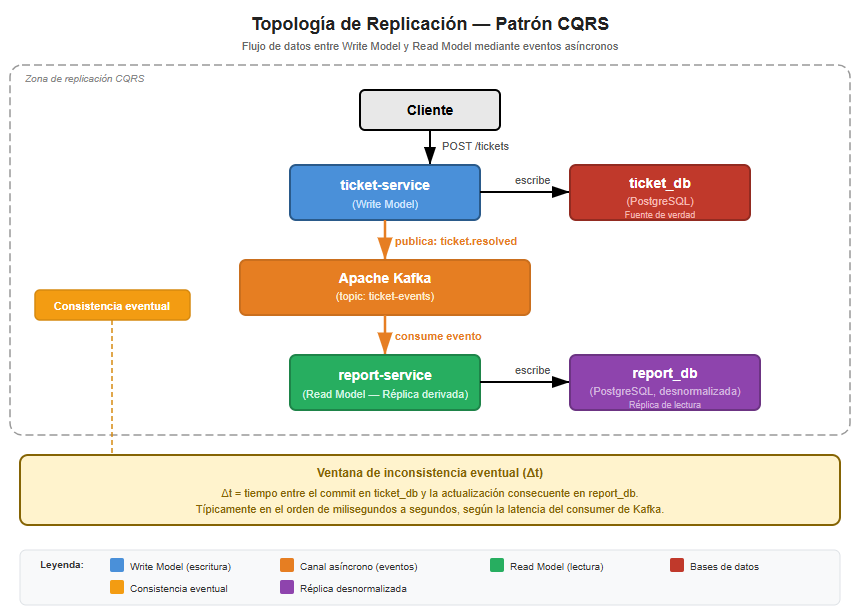
\includegraphics[width=0.85\textwidth]{topologia_cqrs.png}
    \caption{Topología de replicación del patrón CQRS entre \texttt{ticket-service} y \texttt{report-service}, con la ventana de inconsistencia eventual asociada a la propagación asíncrona vía Apache Kafka.}
    \label{fig:topologia_cqrs}
\end{figure}

Como se observa en la Figura~\ref{fig:topologia_cqrs}, el modelo de consistencia resultante de esta topología corresponde a \textbf{consistencia eventual}: en ausencia de nuevas escrituras sobre un ticket dado, \texttt{report\_db} converge eventualmente al mismo estado que \texttt{ticket\_db}, pero no existe garantía de que ambas vistas coincidan en todo instante.

\subsection{Justificación técnica ligada al dominio}
Bajo el marco PACELC, el sistema puede clasificarse como \textbf{PA/EL}. Ante una partición que aísle a \texttt{report-service} del bus de eventos, \texttt{ticket-service} continúa aceptando y persistiendo solicitudes sin degradar su disponibilidad, priorizando \textbf{A} sobre \textbf{C}. En ausencia de partición, la arquitectura evita explícitamente que el cliente espere por la clasificación de IA o por la actualización del modelo de lectura: la respuesta a \texttt{POST /api/v1/tickets} se entrega de inmediato con el identificador del ticket, sin bloquear sobre el resultado de procesos asíncronos, priorizando \textbf{L} sobre \textbf{C}.

Esta decisión es coherente con el dominio de soporte técnico ISP. El dato crítico e inmediato es la existencia trazable del ticket --que el cliente reciba constancia de su reclamo sin demora--, mientras que las métricas derivadas (categoría, prioridad, cumplimiento agregado de SLA) son de naturaleza analítica y toleran una ventana de \textit{staleness} de segundos sin comprometer la operación diaria del servicio técnico. No obstante, esta misma elección introduce una limitación real: mientras persiste la ventana \(\Delta t\), el cumplimiento de SLA reportado por \texttt{report-service} (endpoint \texttt{/api/v1/reports/sla}) puede no reflejar el estado más reciente de los tickets, lo cual se retoma como limitación central en la discusión crítica (Sección 6).

% ============================================================
% 4. EVALUACIÓN DE ALTERNATIVAS
% ============================================================
\section{Evaluación de Alternativas}

\subsection{Alternativas consideradas}
Se contrastan dos alternativas técnicamente realistas frente al modelo actual, seleccionadas por representar los extremos del espectro de consistencia aplicables al mismo problema de sincronización entre el estado operativo del ticket y su vista de reportes.

\textbf{Alternativa 1 -- Consulta síncrona directa.} Consiste en eliminar \texttt{report\_db} como almacén independiente y hacer que \texttt{report-service} consulte directamente \texttt{ticket\_db} en tiempo real, prescindiendo de Kafka como intermediario para este flujo. Es, en esencia, revertir el patrón CQRS.

\textbf{Alternativa 2 -- Replicación multi-líder o por quorum.} Consiste en desplegar múltiples nodos de la base de datos operativa (o migrar a un motor con soporte nativo de quorum) en distintas ubicaciones, permitiendo escrituras concurrentes con resolución de conflictos, escenario plausible si el ISP escalara a múltiples sucursales regionales.

\subsection{Tabla comparativa}
\begin{table}[H]
\centering
\caption{Comparación del modelo actual frente a las alternativas propuestas.}
\label{tab:comparacion}
\small
\begin{tabular}{@{}
    >{\raggedright\arraybackslash}p{4.1cm}
    >{\centering\arraybackslash}p{4.5cm}
    >{\centering\arraybackslash}p{3.1cm}
    >{\centering\arraybackslash}p{4cm}@{}}
\toprule
\textbf{Criterio} & \textbf{Modelo actual (CQRS)} & \textbf{Alt. 1: Síncrona} & \textbf{Alt. 2: Multi-líder} \\
\midrule
Consistencia                  & Eventual                 & Fuerte / lineal   & Eventual con conflictos \\
Disponibilidad                & Alta                     & Media             & Muy alta \\
Latencia (cliente)            & Baja                     & Alta              & Baja \\
Tolerancia a particiones      & Alta                     & Baja              & Muy alta \\
Complejidad de implementación & Media (ya implementado) & Baja              & Alta \\
\bottomrule
\end{tabular}
\end{table}

Como se observa en la Tabla~\ref{tab:comparacion}, la Alternativa 1 mejora la consistencia a costa de acoplar temporalmente al cliente de reportes con la disponibilidad de \texttt{ticket\_db}, sin beneficio proporcional para un dominio donde los reportes no exigen actualidad al milisegundo. La Alternativa 2 mejora la disponibilidad y la tolerancia a particiones, pero introduce una complejidad de implementación --resolución de conflictos, sincronización de relojes-- que no está justificada en la escala actual, de un único ISP sin distribución geográfica.

% ============================================================
% 5. DISCUSIÓN CRÍTICA
% ============================================================
\section{Discusión Crítica}
Retomando la pregunta orientadora, \textit{¿es el modelo de consistencia elegido el óptimo para el dominio del sistema?}, la respuesta es afirmativa con matices. El modelo CQRS con consistencia eventual vía Kafka resulta adecuado para la ruta operativa crítica del cliente --creación y consulta de su propio ticket-- porque prioriza correctamente disponibilidad y baja latencia, tal como exige un servicio de atención de incidencias donde la percepción de rapidez es un factor de calidad de servicio.

Sin embargo, el modelo no es óptimo sin reservas para el subdominio de reportes de cumplimiento de SLA. Mientras persiste la ventana \(\Delta t\), un administrador podría tomar decisiones basadas en métricas de \texttt{report-service} que no reflejan el estado más reciente de los tickets. Esta limitación, ya reconocida implícitamente en la documentación de riesgos del propio PFC, exige mitigaciones concretas:

\begin{enumerate}
    \item \textbf{Transparencia de frescura del dato:} incorporar en cada respuesta de \texttt{report-service} un campo \texttt{lastSyncedAt} que indique hasta qué evento Kafka está actualizada la vista, permitiendo al consumidor juzgar la vigencia del dato antes de actuar sobre él.
    \item \textbf{Separación de la ruta crítica de alertas:} mantener el evento \texttt{sla.breached}, emitido directamente por \texttt{ticket-service}, como camino independiente de \texttt{report\_db} para notificaciones urgentes de incumplimiento, evitando que lo crítico dependa de una vista eventualmente consistente.
    \item \textbf{Acotamiento del \(\Delta t\):} ajustar la configuración del \textit{consumer} de Kafka en \texttt{report-service} (frecuencia de \textit{commit}, \texttt{max.poll.interval.ms}) para convertir la ventana de inconsistencia en un margen medible y predecible, en lugar de una incertidumbre indefinida.
\end{enumerate}

Estas mitigaciones no eliminan la consistencia eventual --que sigue siendo la elección correcta a nivel arquitectónico--, sino que gestionan explícitamente sus consecuencias en el único subdominio donde representan un riesgo real.

% ============================================================
% 6. CONCLUSIONES
% ============================================================
\newpage
\section{Conclusiones}
\begin{enumerate}
    \item El sistema del equipo ACC implementa, mediante el patrón CQRS entre \texttt{ticket-service} y \texttt{report-service}, un modelo de consistencia eventual sostenido por replicación asíncrona basada en eventos de Kafka, distinto del particionamiento funcional (\textit{Database-per-Service}) que rige al resto de microservicios del sistema.
    \item Bajo el marco PACELC, el sistema se clasifica como PA/EL, priorizando disponibilidad ante particiones y latencia en operación normal, decisión coherente con la naturaleza del dominio de soporte técnico ISP.
    \item El modelo es adecuado para la ruta crítica del cliente, pero presenta una limitación identificable en el subdominio de reportes de SLA, para la cual se proponen mitigaciones concretas y viables sin alterar la arquitectura general.
    \item Las alternativas evaluadas --consulta síncrona y replicación multi-líder-- no ofrecen, en la escala actual del proyecto, una mejora que justifique su mayor costo de latencia o de complejidad, respectivamente.
\end{enumerate}

% ============================================================
% 7. DECLARACIÓN DE USO DE IA GENERATIVA
% ============================================================
\section*{Declaración de Uso de Inteligencia Artificial Generativa}
\addcontentsline{toc}{section}{Declaración de Uso de Inteligencia Artificial Generativa}
En cumplimiento de las normativas de honestidad académica de la Universidad Técnica Estatal de Quevedo, se declara el uso de la herramienta ChatGPT como apoyo en la elaboración del presente informe, específicamente en la verificación de referencias académicas, el formato LaTeX y su mejora en lo que respecta a estructura y redacción. El análisis conceptual, la caracterización del modelo del PFC y las conclusiones son de autoría del estudiante.

% ============================================================
% REFERENCIAS
% ============================================================
\clearpage
\printbibliography[title={Referencias}]

\end{document}
